\documentclass[12pt]{article}         %% What type of document you're writing.


%%%%% Preamble

%% Packages to use
\usepackage[margin=1.1in]{geometry}
\usepackage{amsmath,amsfonts,amssymb}   %% AMS mathematics macros
\usepackage[utf8]{inputenc}
\usepackage{chngcntr}
\usepackage{graphicx}
\counterwithin*{equation}{section}

%% Title Information.

\title{Assignment 1 \\ OCS}
\author{Marko Ivančić \and Mauro Jurada}
\date{2 November 2019}           %% By default, LaTeX uses the current date

%%%%% The Document

\begin{document}

\maketitle


\section{Characterization of Functions}
%% 1
\begin{equation}
	f(x,y) = 2x^3 - 6y^2 + 3x^2 y
\end{equation}

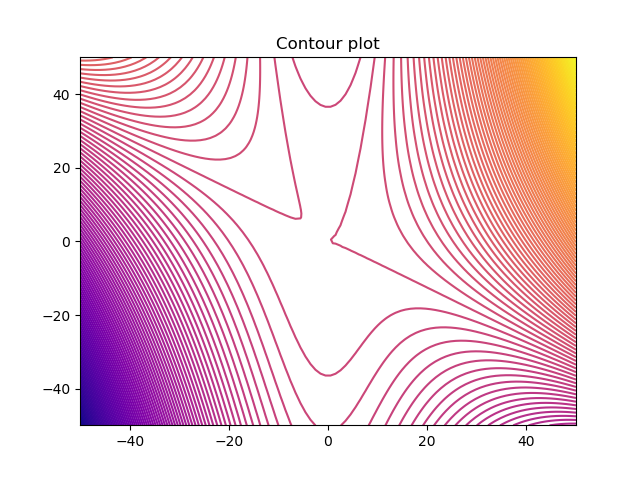
\includegraphics[width=0.5\textwidth]{Figure_1}
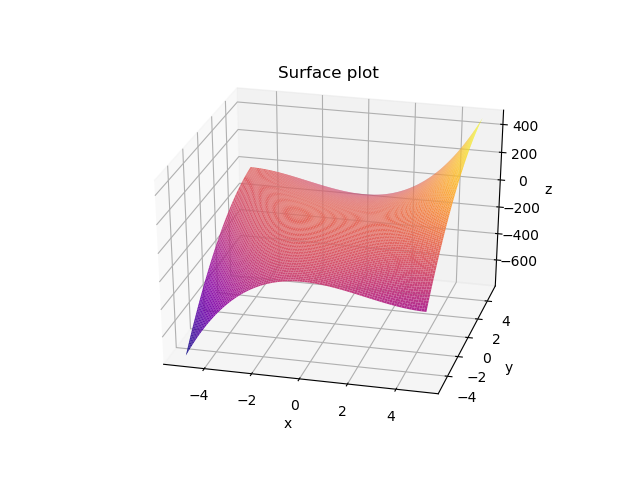
\includegraphics[width=0.5\textwidth]{Surface_1}

$$
\frac {\partial f}{\partial x} = 6x^2 + 6xy \quad\Rightarrow 
	\left\{
	\begin{aligned}
		\frac {\partial^2 f}{\partial x^2}&=12x+6y\\ 
		\frac {\partial^2 f}{\partial y \partial x}&=6x
	 \end{aligned} 
	 \right.
$$

$$
\frac {\partial f}{\partial y} = -12y+3x^2 \quad\Rightarrow 
	\left\{
	\begin{aligned}
		\frac {\partial^2 f}{\partial y^2}&=-12\\ 
		\frac {\partial^2 f}{\partial x \partial y}&=6x
	 \end{aligned} 
	 \right.
$$

Stationary points:

$$
6x^2+6xy=0 \quad\Rightarrow x^2+xy=0 \quad\Rightarrow x(x+y)=0 %% clarification
$$
$$
3x^2-12y=0 \quad\Rightarrow x^2-4y=0
$$
$$
\begin{aligned}
-xy-4y&=0\\
y(x+4)&=0\\
x_1&=0, \quad y_2=0\\
x_2&=-4 \quad\Rightarrow 16-4y=0\\
y_2&=4
\end{aligned}
$$
\begin{gather}
\nabla^2 f(x,y) = 
  \begin{bmatrix}
  12 X + 6Y &
   6X\\
   6X &
   -12 
   \end{bmatrix}
    \nonumber %%no numerating the eq
\end{gather}


$$
\begin{aligned}
\det\left(\nabla^2 f(x,y)\right)=&-12*(12x+6y) - 36x^2= -144x-72y-36x^2\\
1)\: &x_1=0, y_1=0\\
&det=0 \\  \quad\implies \text{Saddle point}%% ??????????????????????????????????????????????????????????????????????????????
2)\: &x_2=-4, y_2=4\\
&det=576-288-576=-288 \quad\implies \text{Saddle point}
\end{aligned}
$$\\

%% 2
\begin{equation}
	f(x,y) = (x - 2y)^4 + 64xy
\end{equation}

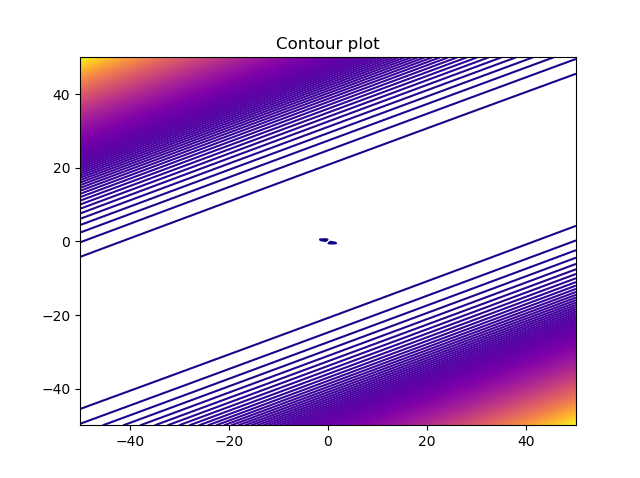
\includegraphics[width=0.5\textwidth]{Figure_2}
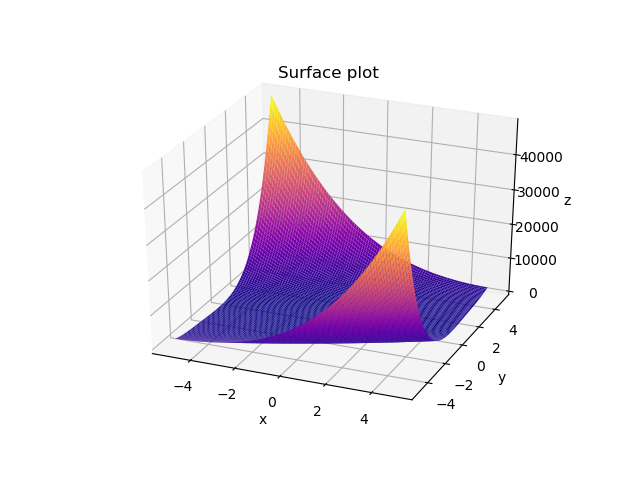
\includegraphics[width=0.5\textwidth]{Surface_2}

$$
\frac {\partial f}{\partial x} = 4(x-2y)^3 + 64y \quad\Rightarrow 
	\left\{
	\begin{aligned}
		\frac {\partial^2 f}{\partial x^2}&=12(x-2y)\\
		\frac {\partial^2 f}{\partial y \partial x}&=-24(x-2y)^2 +64
	 \end{aligned} 
	 \right.
$$

$$
\frac {\partial f}{\partial y} = -8(x-2y)^3 +64x \quad\Rightarrow 
	\left\{
	\begin{aligned}
		\frac {\partial^2 f}{\partial y^2}&=-48(x-2y)^2\\ 
		\frac {\partial^2 f}{\partial x \partial y}&=-24(x-2)^2 +64
	 \end{aligned} 
	 \right.
$$\\

Stationary points:

$$
4(x-2y)^3 +64y=0  \quad\Rightarrow 
(x-2y)^3 + 16y=0
$$
$$
-8(x-2y)^3+64x=0  \quad\Rightarrow
(x-2y)^3 -8x=0
$$

$$
\begin{aligned}
8x+16y&=0\\
x+2y&=0\\
x&=-2y
\end{aligned}
$$
$$
\begin{aligned}
(-2y -2y)^3 +16y&=0\\
-64y^3 +16y&=0\\
4y^3 -y&=0\\
y(4y^2 -1)&=0\\
y(2y-1)(2y+1)&=0\\
1)\: x_1=&\:0,\quad y_1=0\\
2)\: x_2=&\: -\!1,\quad y_2=\frac{1}{2}\\ 
3)\: x_3=&\:1,\quad y_3=-\frac{1}{2}
\end{aligned}
$$

\begin{gather}
\nabla^2 f(x,y) = 
  \begin{bmatrix}
  12 (X - 2Y)^2 &
  -24 (X - 2Y)^2 + 64\\
  -24 (X - 2Y)^2  +64 &
  48 (X - 2Y)^2 
   \end{bmatrix}
    \nonumber
\end{gather}


$$
\begin{aligned}
\det&\left(\nabla^2 f(x,y)\right)=-12*48(x-2y)^4 -(64-24(x-2y)^2)^2\\
1)\: x_1&=0, \quad y_1=0\\
\det&=12*48(0-0) - (64-24(0-0)^2)^2 =64^2 < 0   \quad\implies \text{Saddle point}\\
2)\: x_2&=-1, \quad y_2=\frac{1}{2}\\
\det&=12*48(-1-1)^4 -(46-24(-1-1)^2)^2=(576*(-16)-32^2)<0 \quad\implies \text{Saddle point}\\
3)\: x_3&=1, \quad y_3=-\frac{1}{2}\\
\det&=12*48*2^4 -(64 -24*2^2)^2 = 576*16-32^2>0 \quad \&\& \quad \frac {\partial^2 f}{\partial x^2} > 0 \quad\implies \text{Global Minimum}\\
\end{aligned}
$$
 \pagebreak

%% 3
\begin{equation}
	f(x,y) = 2x^2 +3y^2 - 2xy + 2x - 3y
\end{equation}

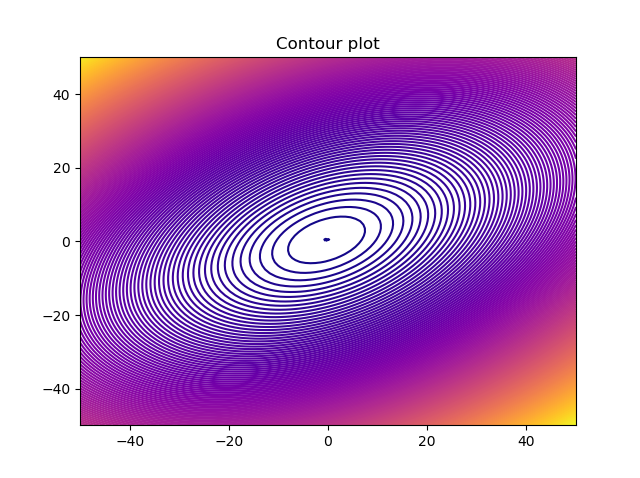
\includegraphics[width=0.5\textwidth]{Figure_3}
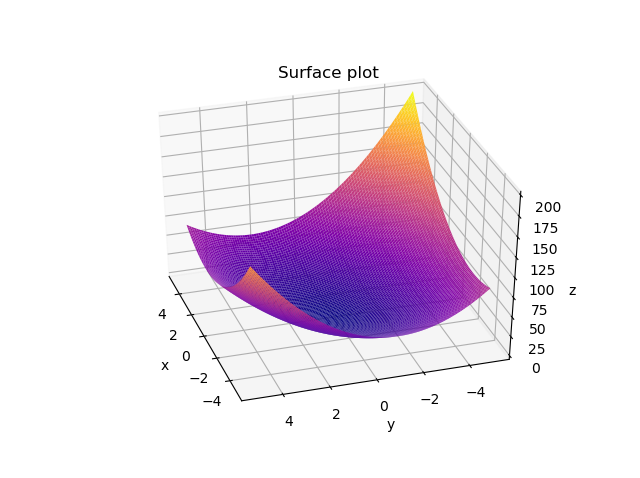
\includegraphics[width=0.5\textwidth]{Surface_3}

$$
\frac {\partial f}{\partial x} = 4x-2y+2 \quad\Rightarrow 
	\left\{
	\begin{aligned}
		\frac {\partial^2 f}{\partial x^2}&=4\\
		\frac {\partial^2 f}{\partial y \partial x}&=-2
	 \end{aligned} 
	 \right.
$$
$$
\frac {\partial f}{\partial x} = 6y-2x-3 \quad\Rightarrow 
	\left\{
	\begin{aligned}
		\frac {\partial^2 f}{\partial x^2}&=6\\
		\frac {\partial^2 f}{\partial y \partial x}&=-2
	 \end{aligned} 
	 \right.
$$

Stationary points:

$$
\begin{aligned}
4x-2y+2&=0 \quad\Rightarrow 2x-y+1=0 \quad\Rightarrow y=2x+1\\
6y-2x-3&=0\\
&6(2x+1) -2x-3=0\\
&10x-3=0\\
&x=\frac{-3}{10}\\
&y=2\frac{-3}{10} +1 = \frac{2}{5}
\end{aligned}
$$

\begin{gather}
\nabla^2 f(x,y) = 
  \begin{bmatrix}
   4 &
   -2\\
   -2 &
   6 
   \end{bmatrix}
   \nonumber
\end{gather}

$$
\det\left(\nabla^2 f(x,y)\right) = 4*6-(-2)^2=24-4=20 >0  \quad \&\& \quad 4 > 0 \quad\implies \text{Strict Global Minimum}\\ % ???????????????
$$\\


%% 4
\begin{equation}
	f(x,y) = \ln(1 + \dfrac{1}{2}(x^2 +3y^2))
\end{equation}

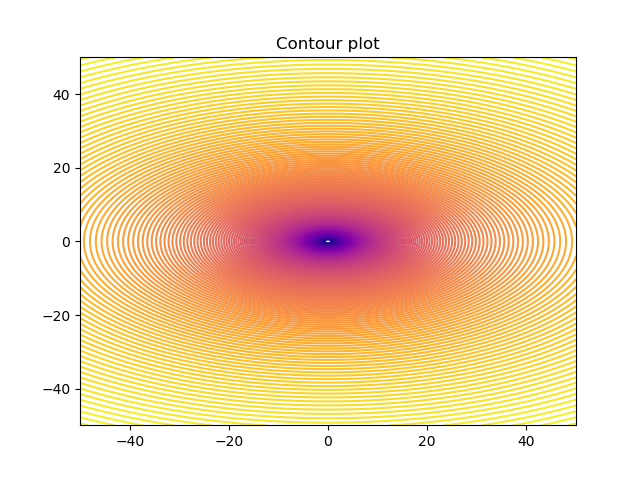
\includegraphics[width=0.5\textwidth]{Figure_4}
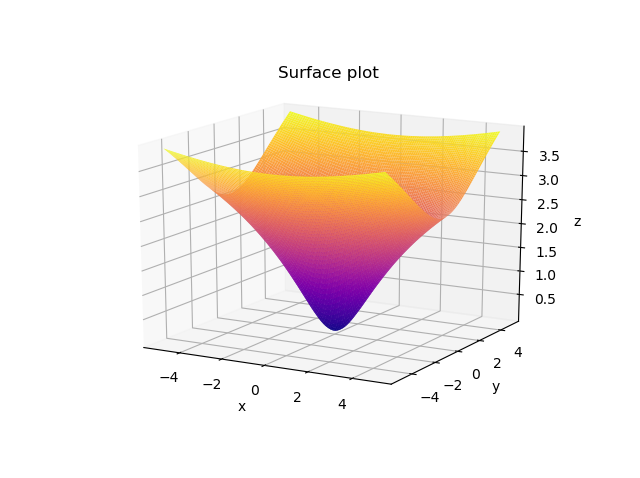
\includegraphics[width=0.5\textwidth]{Surface_4}

$$
\begin{aligned}
\frac {\partial f}{\partial x} = \frac{1}{1+\frac{1}{2}(x^2+3y^2)}x= \frac{x}{\frac{1}{2}(2+x^2+3y^2)}=\frac{2x}{2+x^2+3y^2}\\
\implies 
	\left\{
	\begin{aligned}
		\frac {\partial^2 f}{\partial x^2}&=\frac{2(2+x^2+3y^2)-2x(2x)}{(2+x^2+3y^2)^2}=
		 	\frac{4-2x^2+6y^2}{(2+x^2+3y^2)^2} \\
		\frac {\partial^2 f}{\partial y \partial x}&=\frac{0(2+x^2+3y^2)-2x(6y)}{(2+x^2+3y^2)^2}=
		 	\frac{-12xy}{(2+x^2+3y^2)^2} 
	 \end{aligned} 
	 \right.
\end{aligned}
$$

$$
\begin{aligned}
\frac {\partial f}{\partial x} = \frac{1}{1+\frac{1}{2}(x^2+3y^2)}3y= \frac{3y}{\frac{1}{2}(2+x^2+3y^2)}=\frac{6y}{2+x^2+3y^2}\\
\implies 
	\left\{
	\begin{aligned}
		\frac {\partial^2 f}{\partial x^2}&=\frac{6(2+x^2+3y^2)-6y(6y)}{(2+x^2+3y^2)^2}=
		 	\frac{12+6x^2-18y^2}{(2+x^2+3y^2)^2} \\
		\frac {\partial^2 f}{\partial y \partial x}&=\frac{0(2+x^2+3y^2)-6y(2x)}{(2+x^2+3y^2)^2}=
		 	\frac{-12xy}{(2+x^2+3y^2)^2} 
	 \end{aligned} 
	 \right.
\end{aligned}
$$

Stationary points:

$$
\frac{2x}{2+x^2+3y^2}=0 \quad\Rightarrow x=0\\
$$
$$
\frac{6y}{2+x^2+3y^2}=0 \quad\Rightarrow y=0\\
$$
\begin{gather}
\nabla^2 f(x,y) = 
  \begin{bmatrix}
   \dfrac{4 - 2X^2 +6Y^2}{(2 + X^2 + 3Y^2)^2} &
   \dfrac{-12XY}{(2 + X^2 + 3Y^2)^2}\\
   \dfrac{-12XY}{(2 + X^2 + 3Y^2)^2} &
   \dfrac{12 + 6X^2 - 18Y^2}{(2 + X^2 + 3Y^2)^2} 
   \end{bmatrix}
    \nonumber
\end{gather}

$$
\det\left(\nabla^2 f(x,y)\right)=\frac{4-2x^2+6y^2}{(2+x^2+3y^2)^2} * \frac{12+6x^2-18y^2}{(2+x^2+3y^2)^2} - \frac{-12xy}{(2+x^2+3y^2)^2} *  \frac{-12xy}{(2+x^2+3y^2)^2}
$$
$$
1) x=0, \quad y=0 \quad\Rightarrow det=\frac{4}{4}*\frac{12}{4}-\frac{0}{4}*\frac{0}{4} > 0  \quad \&\& \quad \frac{4}{4} > 0 \quad\implies \text{Strict Global Minimum}
$$

%Consider the two points $(-1,16)$ and $(3,1)$.  quation $y = m x + b$ through the two points, and
%Section fits a exponential equation $y = A e^{k x}$
% $y$-intercept $b$ of the line.


\section{Numerical Gradient Approximation}


\begin{equation}
	\nabla_x f(x,y) \approx \dfrac{f(x + \epsilon, y) - f(x - \epsilon, y)}{2\epsilon}
\end{equation}

\begin{equation}
	\nabla_x f(x,y) \approx \dfrac{f(x, y + \epsilon) - f(x, y - \epsilon)}{2\epsilon}
\end{equation}

1.1)\\
$$
\begin{aligned}
(x,y) &= (1, -4)\\
\nabla_x f(x,y) &= -17.999998000007622\\
\nabla_y f(x,y) &= 51.00000000000904\\
\frac {\partial f}{\partial x} &= -18\\
\frac {\partial f}{\partial y} &= 51\\\\
\end{aligned}
$$

1.2)\\
$$
\begin{aligned}
(x,y) &= (0, 2)\\
\nabla_x f(x,y) &= -128.00001600004407\\
\nabla_y f(x,y) &= 512.00012799994\\
\frac {\partial f}{\partial x} &= -128\\
\frac {\partial f}{\partial y} &= 512\\\\
\end{aligned}
$$

1.3) \\
$$
\begin{aligned}
(x,y) &= (1, 3)\\
\nabla_x f(x,y) &= -1.7763568394002505e-12\\
\nabla_y f(x,y) &= 12.9999999999999\\
\frac {\partial f}{\partial x} &= 0\\
\frac {\partial f}{\partial y} &= 13\\\\
\end{aligned}
$$

1.4)\\
$$
\begin{aligned}
(x,y) &= (-4, 4)\\
\nabla_x f(x,y) &= -0.12121211996918291\\
\nabla_y f(x,y) &= 0.3636363631356332\\
\frac {\partial f}{\partial x} &= -0.12121212\\
\frac {\partial f}{\partial y} &= 0.363636363\\\\
\end{aligned}
$$


\section{Vectors, Norms and Matrices}


\subsection{}
$\vert$$\vert$.$\vert$$\vert_{1/2}$ is not a norm because it violates the third rule for norms, triangle inequality, for vectors x=(1,0) and y=(0,1)

$$
\begin{aligned}
||x+y||&\leq ||x|| + ||y||\\
||(1, 0) + (0, 1)||&\leq ||(1, 0)|| + ||(0, 1)||\\
||(1, 1)||&\leq ||(1, 0)|| + ||(0, 1)||\\
(\sqrt{1} + \sqrt{1})^2&\leq (\sqrt{1} + \sqrt{0})^2 + (\sqrt{0} + \sqrt{1})^2\\
2^2 &\leq 1^2 + 1^2\\
4 &\leq 2\\
\end{aligned}
$$

\subsection{}
To prove this inequality we will use the triangle inequality
$$
\begin{aligned}
||a + b||&\leq ||a|| + ||b||\\
\text{Replace a and b}\\ a &= x-y\\ b &= y-z\\ \text{then}\\
||x - y + y - z||&\leq ||x-y|| + ||y-z||\\
||x - z||&\leq ||x-y|| + ||y-z||\\
\end{aligned}
$$





\section{Matrix Calculus}

\begin{equation}
	f(x) = \dfrac{1}{2}\Vert Ax - b\Vert^2 \quad\text{for}\; x\in \mathbb{R} ^n ,b\in \mathbb{R}^m \;\text{and}\; A\in\mathbb{R}^{m*n}
\end{equation}


$$
\begin{aligned}
\text{We write the equation in vector form:}\\
f(x) = \dfrac{1}{2}||
  \begin{bmatrix}
 \sum_{j=0}^{n}a_{0j}x_j - b_0\\
\vdots\\
  \sum_{j=0}^{n}a_{mj}x_j - b_m
   \end{bmatrix}
||^2\\\\
\text{The square root is cancelled by power of 2}\\
f(x) = \dfrac{1}{2}\sum_{i=0}^{m}(\sum_{j=0}^{n}a_{ij}x_j - b_i)^2\\\\
\text{we derive the bracket and whats inside the bracket}\\
\frac {\partial f(x)}{\partial x_k} = \sum_{i=0}^{m}(\sum_{j=0}^{n}a_{ij}x_j - b_i)a_{ik}\\
\end{aligned}
$$
$$
\text{Linear form: }\\
	\frac {\partial f(x)}{\partial x}  = A^t(Ax - b)
$$\\
\begin{equation}
	f(\alpha) = \dfrac{1}{2}||A(x - \alpha y) - b||^2
\end{equation}
\\
\\
$$
\begin{aligned}
\text{We write the equation in vector form:}\\
f(x) = \dfrac{1}{2}||
  \begin{bmatrix}
 \sum_{j=0}^{n}a_{0j}(x_j + \alpha y_j) - b_0\\
\vdots\\
  \sum_{j=0}^{n}a_{mj}(x_j + \alpha y_j) - b_m
   \end{bmatrix}
||^2\\\\
\text{The square root is cancelled by power of 2}\\
f(x) = \dfrac{1}{2}\sum_{i=0}^{m}(\sum_{j=0}^{n}a_{ij}(x_j + \alpha y_j) - b_i)^2\\\\
\text{we derive the bracket and whats inside the bracket}\\
\frac {\partial f(\alpha)}{\partial \alpha} = \sum_{i=0}^{m}[ ( \sum_{j=0}^{n}(a_{ij}x_j +a_{ij}y_j\alpha) - b_i)(\sum_{j=0}^{n}a_{ij}y_j]\\
\end{aligned}
$$
$$
\text{Linear form: }\\
	\frac {\partial f(\alpha)}{\partial \alpha} = y^tA^t(A(x +\alpha y) - b)
$$\\

%%$$
	%%16 = A e^{(-\ln(2))(-1)} = A e^{\ln{2}} = 2 A
	.
%%$$


\section{Student Task Selection Problem}


\end{document}

